\chapter{Ausblick} % Main chapter title
\label{chapter6:Ausblick} % Change X to a consecutive number; for referencing this chapter elsewhere, use \ref{ChapterX}

In diesem Kapitel wird der weitere Verlauf des MVB-Sniffers besprochen, und dabei Aufgaben des Sniffers die in der folgenden Bachelorarbeit, implementiert werden sollen angesprochen.
Das Kapitel ist in die Hauptkomponenten des Sniffers unterteilt.


\section{Hardware FPGA}
\label{sec:AusblickHardwareFPGA}
In der Weiterentwicklung des Sniffers soll die Implementierung des Puffers keine Fehler mehr verursachen. Es ist Festzustellen wo die Fehlerquelle ist, und diese zu beheben.

Die Konfigurierung des FPGA kann so ausgebaut werden, dass ein Senden der Daten nur dann geschehen soll, wenn der empfangende Mikrocontroller bereit ist und dies zum Beispiel mit einem Handshake signalisiert. Dabei sollen Daten, welche in dieser Zeit decodiert werden, in einen weiteren Puffer geschrieben werden und sobald der Mikrocontroller bereit ist, sollen diese übermittelt werden.

Es ist vorgesehen, dass das FPGA zusätzlich zu den Daten einen Zeitstempel übermittelt, damit weitere Auswertungen der Daten aussagekräftiger werden.

Eine weitere Idee ist es, die komplette Decodierung und Auswertung des Manchestersignals im FPGA durchzuführen und dem Mikrocontroller nur den Payload, mit der Info, ob es ein Master- oder Slave-Frame ist, weiterzugeben. Dabei wäre es notwendig, einen Buffer anzulegen, welcher je nach Telegramm veränderlich gross ist. 

Wie in Abbildung \ref{fig:FPGAanalyse} zu sehen ist, wurde nur gerade 4 \% des FPGA für Logik des Sniffers benötigt. Hier stellt sich die Frage, ob nicht allenfalls ein kleinerer FPGA in Betracht gezogen werden kann, um Einsparungen in Ausgaben und Platz erzielen zu können.\\

\begin{figure}[H]
    \centering
    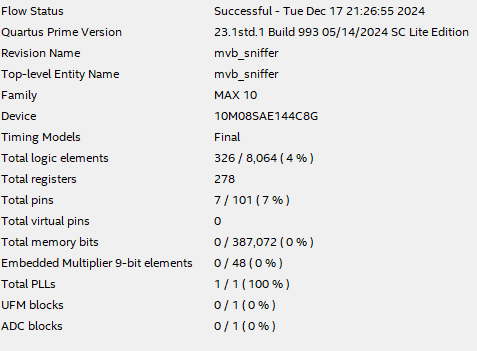
\includegraphics[width=0.55\linewidth]{Figures/Chap6/FPGA/quartus_analyzer.PNG}
    \caption{Analyse nach Synthetisierung des VHDL-Codes}
    \label{fig:FPGAanalyse}
\end{figure}



\section{Firmware ESP32-S3}
\label{sec:AusblickFirmwareESP32}
Aufgrund der Limitierung der SPI-Schnittstelle auf dem ESP32-S3 wird geprüft, den verwendeten Mikrocontroller durch eine Alternative mit echter Hardware-SPI-Peripherie zu ersetzen. Diese Anpassung würde eine effizientere und niedriger latente Kommunikation mit dem angeschlossenen FPGA ermöglichen. Der ersetzende Mikrocontroller soll gleichermassen fähig sein, Bluetooth Low Energy sowie die Paket-Length-Extention und den 2 M PHY zu verwenden.

Darüber hinaus sind Optimierungen der Software-Performance vorgesehen. Ziel ist es, das Programm auf die neue Entwicklungsumgebung schnell anzupassen und das unterstützte Real Time Operating System zu verwenden. Das Programm soll mit bekannten Profiling-Programmen analysiert und der Code optimiert werden. Damit soll ein effizienteres und stabileres System sichergestellt werden.

Ein weiterer Schwerpunkt liegt auf der Entwicklung und Integration erweiterter Funktionen. Filterfunktionen für Telegramme. Diese sollen eine präzisere Analyse und Verarbeitung von eingehenden Daten ermöglichen, wodurch die Anwendbarkeit des Systems für spezifische Anforderungen weiter verbessert wird.

Abschliessend ist die Implementierung eines benutzerfreundlichen Interfaces geplant. Dieses soll sowohl die Konfiguration des Sniffers, also die Einstellung von Filtern, als auch das Empfangen und Visualisieren von Telegrammen vereinfachen. Die Implementierung des Interfaces soll auf dem Endgerät stattfinden, wie beispielsweise einem Laptop. Dadurch wird die Benutzererfahrung optimiert und die Handhabung intuitiver gestaltet.




\section{Hardware Design}
\label{sec:AusblickHardware}
Für die Weiterentwicklung des MVB-Sniffers hardwareseitig sind grundlegende Anpassungen und Erweiterungen vorgesehen. Aufgrund der identifizierten Probleme mit der SPI-Schnittstelle wird der Wechsel zu einem neuen Mikrocontroller stark in Betracht gezogen. Die Auswahl eines Mikrocontrollers, der die spezifischen Anforderungen des Projekts besser erfüllt, hat hohe Priorität, um die Kommunikationsprobleme zu lösen und den Sniffer auf dem realen MVB verwenden zu können.

Zusätzlich ist die Integration eines Akkus geplant, um den Umgang mit dem Sniffer mobiler und unabhängiger von externen Stromversorgungen zu machen. Je nach Wahl des neuen Mikrocontrollers könnte es erforderlich sein, ein Bluetooth-Modul zu integrieren, um eine drahtlose Kommunikation weiterhin beizubehalten und einen weiteren wesentlichen Vorteil gegenüber den erhältlichen Produkten zu bieten.

Aus diesen Gründen werden nochmals schematische Anpassungen und Erweiterungen notwendig sein, um die neuen Komponenten und deren Funktionalität korrekt im Schema einzupflegen. Diese Anpassungen sollten so früh wie möglich geschehen, um den Übergang zum PCB-Design möglichst rasch zu machen, da dieser eine gewisse Zeit in Anspruch nimmt, wie sich im Rahmen der Projektarbeit gezeigt hat. Das Ziel ist es, im Verlauf der Bachelorarbeit so schnell wie möglich ein PCB zu haben, damit mit der finalen Sniffer-Hardware gearbeitet werden kann. Dadurch kann die Software für die Visualisierung und Auswertung unter echten Bedingungen entwickelt werden und Überraschungen hinsichtlich neuer Komponenten kann frühzeitig reagiert werden. Zudem kann die bisher entwickelte Firmware und die FPGA-Hardwarebeschreibungssprache validiert werden und wo nötig angepasst werden.
